% \newpage
\section{Integrazione con codice esterno}\label{subsec:mysubsection}
Elixir è offre completa Interoperabilità
con il codice Erlang, e si ha a disposizione tutta la gamma di librerie
già sviluppate per Erlang, molte librerie non vengono riscritte in Elixir
potendo usare quelle già ben testate sulla piattaforma Erlang.

Non tutto può essere implementato in modo efficiente
usando Erlang ed Elixir, basti pensare che l'immutabilità dei dati
porta molti vantaggi per lo sviluppo concorrenziale, ma porta altri
svantaggi. Nella seguente lista vengono messi in evidenza alcune
lacune che presenta la Erlang VM.

\begin{itemize}
	\item \textbf{Matematica avanzata}: La VM non è stata progettata per operazioni
	intensive di calcolo numerico. Se l'applicazione dipende dal calcolo di
	statistiche si possono riscontrare delle limitazioni.
	\item \textbf{Soluzioni algoritmiche tramite matrici}: L'implementazione
	nativa di matrici in Elixir usa liste di liste, che non è una rappresentazione
	efficiente delle matrici multidimensionali. Inoltre la mancanza di mutabilità
	porta a fare una copie di matrici anche grandi per semplici operazioni.
	\item \textbf{Command Line Applications}: La VM impiega circa 0.3 secondi
	per l'avvio e lo spegnimento anche per l'hardware moderno, dopotutto Erlang
	è stato progettato per sistemi a lungo termine, ciò non porta ad essere
	la scelta ottimale per una CLI.
\end{itemize}

Ci possono essere un sacco di insiemi di problemi in cui Elixir
non è la soluzione migliore, ma può risultare utile comunque
usare Elixir e risolvere problemi in cui non è adatto
con un codice esterno scritto in un altro linguaggio adatto
alle esigenze specifiche.
In particolare Elixir può comunicare con altri linguaggi
in 3 modi diversi:

\begin{itemize}
	\item NIF (Native implemented functions): L'applicazione può condividere lo stesso
	spazio degli indirizzi di memoria.
	Una NIF è una funzione scritta in C/C++, viene compilata
	come libreria condivisa e caricata all'avvio dell'applicazione.
	\item Ports: Elixir può invocare processi esterni alla macchina
	virtuale, è una forma di Interprocess communication (IPC).
	\item Erlang Distribution Protocol: Si può comunicare con
	processi esterni anche su macchine differenti
	attraverso il protocollo di distribuzione fornito per distribuire
	un applicazione su più nodi scalando orizzontalmente un sistema,
	questo metodo non è stato sperimentato in questo luogo.
\end{itemize}


%------------------------  NIF ---------------------------------

\subsection{Interoperabilità tramite NIF}

Le funzioni native NIF, permettono di caricare codice esterno
nello stesso spazio di memoria della Erlang VM. 
Questa strategia di interoperabilità porta a dei benefici
sulle performance elevati per alcune tipologie di calcolo
come quello matematico.
Erlang fornisce un API nel file header
"erl\_nif.h" \cite{Erlanger73:online} consentendo 
di scrivere funzioni C e poter essere chiamate direttamente
dal programma Elixir/Erlang.

Queste funzioni C devono essere compilate come librerie condivise,
shared object(.so in linux). Viene riportato
nell' esempio \ref{lst:example_nif} il codice NIF
che stampa "Hello from C"\cite{adoptingElixirchap7pag126}.

\begin{lstlisting}[language=cpp,captionpos=b,
	caption={Funzione Nif},label={lst:example_nif}]
#include "string.h"
#include "erl_nif.h"

static ERL_NIF_TERM hello(ErlNifEnv* env,int argc,
                          const ERL_NIF_TERM argv[]) {
  ErlNifBinary *output_binary;
  enif_alloc_binary(sizeof "Hello from C", output_binary);
  strcpy(output_binary->data, "Hello from C");
  return enif_make_binary(env, output_binary);
}

static ErlNifFunc nif_funcs[] = {
  {"hello", 0, hello},
};

ERL_NIF_INIT(Elixir.ElixirNif, nif_funcs, NULL, NULL, NULL, NULL)
	
\end{lstlisting}

Si può compilare con il compilatore \textbf{gcc}
con il seguente comando:

\begin{lstlisting}[language=none]
gcc -o <destination-directory>/hello.so -shared -fpic \\
  -I $ERL_ROOT/usr/include <file-directory>/hello.c
\end{lstlisting}

Una volta compilata la libreria si può caricare all'interno del
modulo nel quale si vuole usare la funzione come
nell'esempio \ref{lst:elixir_nif}.

\begin{lstlisting}[language=elixir, caption={Caricamento NIF},
	captionpos=b,label={lst:elixir_nif}]
defmodule ElixirNif do
  @on_load :load_nif

  def load_nif do
	:ok = :erlang.load_nif(String.to_charlist("priv/elixir_nif"), 0)
  end

  def hello do
    "Hello from Elixir"
  end
end
\end{lstlisting}

L'annotazione @on\_load :load\_nif dice alla VM di eseguire load\_nif/0
all'avvio dell'applicazione.
La funzione hello necessita di essere ridefinita anche in Elixir,
così da permettere che la chiamata non fallisca nonostante qualche
eventuale errore nel caricamento della NIF.

Nonostante è uno dei metodi più efficienti per eseguire codice C/C++,
questo metodo ha degli svantaggi \cite{Erlanger73:online}:

\begin{itemize}
	\item Una funzione nativa che va in crash, farà andare in crash l'intera
	VM, per questo è sconsigliato usare questo metodo se non strettamente necessario,
	questo rischio va contro la filosofia di Erlang nella costruzione di sistemi
	fault-tolerant.
	\item Una funzione nativa implementata erroneamente può causare
	un'inconsistenza dello stato interno della VM, che può portare 
	al crash della VM o a comportamenti imprevisti della VM in 
	qualsiasi momento dopo la chiamata alla funzione nativa.
	\item Una funzione nativa che viene eseguita a lungo degrada la
	responsività della VM e può portare a comportamenti strani, che possono
	portare a un utilizzo della memoria eccessivo.
\end{itemize}

Un esempio più complesso dell'utilizzo di una NIF è riportato
nel paragrafo \ref{subsec:NIF_cpp}.
%------------------------ PORT -------------------

\subsection{Interoperabilità con Port}

Il meccanismo Port è un alternativa più sicura per
integrare codice esterno. Ogni Port comunica con un
processo esterno del sistema operativo.
In questo caso se il Port termina, il codice Elixir
viene notificato con un messaggio e può agire di conseguenza
continuando permettendo di avere un interazione robusta
in confronto alle NIF. Per esempio un Segmentation fault
in un processo che comunica tramite Port non porta alla
terminazinoe della VM. Per questi motivi prima di integrare
codice esterno tramite NIF conviene sempre prendere in considerazione
il meccanismo Port prima, per non perdere i benefici dati dalla
piattaforma Erlang. In Figura \ref{fig:port_communication}
si può vedere come la macchina virtuale comunica con un
processo esterno attraverso questo meccanismo, il processo che
crea il Port viene chiamato Processo connesso, a questo punto
si comunica con il processo connesso in due modi:
\begin{enumerate}
	\item Tramite l'API fornita da Elixir \cite{Port—Eli85:online},
	si possono mandare messaggi in maniera sync.
	\item Tramite le primitiva send/2 si può inviare un
	messaggio al processo in maniera asincrona.
\end{enumerate}

\begin{figure}[!htp]
    \centering
    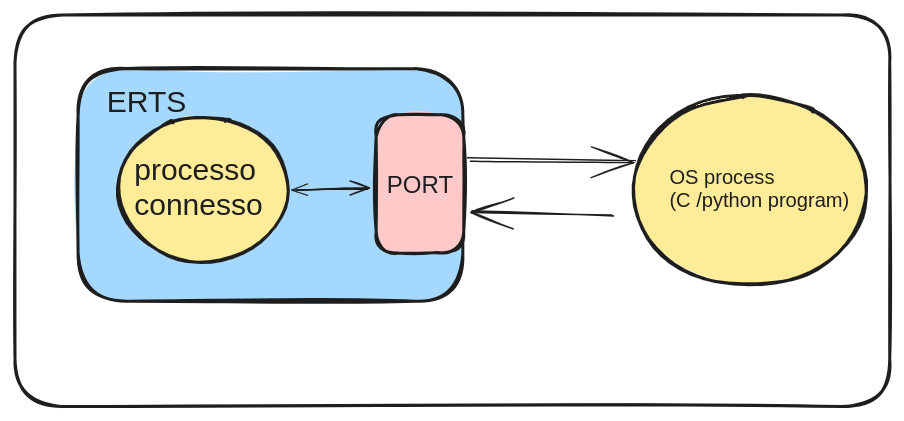
\includegraphics[keepaspectratio=true,scale=0.35]{images/port_communication.png}
	\caption{Comunicazione con Port \cite{ErlangPo88:online}}
  	\label{fig:port_communication}
\end{figure}

Viene riportato nell'esempio \ref{lst:port_example},
un apertura di una Port per il comando "echo" di bash.

\begin{lstlisting}[language=elixir,captionpos=b
	caption={Comando echo con Port},label={lst:port_example}]

iex> path = System.find_executable("echo")
iex> port = Port.open({:spawn_executable, path},
...  [:binary, args: ["hello world"]])
iex> flush()
{#Port<0.1380>, {:data, "hello world\n"}}	
\end{lstlisting}

Un esempio di uso più complesso si trova nel paragrafo \ref{subsec:port_cpp}.
\subsubsection{La libreria ErlPort}
Un caso di particolare interesse può essere la comunicazione
tra Elixir e python, per 
trarre vantaggio dalla vasta gamma di librerie offerte dalla
community degli sviluppatori di Python.

Proprio in quest'ambito la libreria \textbf{ErlPort} ci consente
di avviare istanze python da Elixir, una libreria open source
costruita grazie al meccanismo Port, in grado di interagire con
il linguaggio python o ruby. Non si entra in dettaglio di
questa libreria.
ErlPort permette a Erlang e il linguaggio esterno di scambiare
dati, invocare funzioni l'uno sull'altro e gestire lo stato
condiviso in modo trasparente.
Questo facilita l'integrazione di applicazioni scritte in
Erlang con applicazioni scritte in python o ruby e consente di
sfruttare le specifiche capacità di ciascun linguaggio
all'interno di un unico sistema.

Ad esempio, con ErlPort, è possibile utilizzare Python
per elaborare dati complessi o interfacce utente,
mentre si sfruttano le potenti capacità di concorrenza di
Erlang per gestire la comunicazione di rete o i
processi di calcolo intensivo.

Inoltre con questa libreria non ci si deve preoccupare
della scelta di codifica e decodifica dei dati, ErlPort
infatti utilizza il protocollo di serializzazione di Erlang,
noto come External Term Format (ETF), per la codifica e
la decodifica dei dati scambiati tra Erlang e altri
linguaggi di programmazione.

Non si entra in dettaglio della libreria, però questo è
uno dei modi vantaggiosi per comunicare con python, e
in futuri usi tale libreria è da tenere in considerazione per
processare dati non convenienti per la VM beam.


